\documentclass[10pt]{article}

\usepackage{amsfonts}
\usepackage{amsmath}
\usepackage{amssymb}
\usepackage{amsthm}
\usepackage{booktabs}
\usepackage{mathrsfs}
\usepackage{graphicx}
\usepackage{cite}
\usepackage{times}
\usepackage{url}
\usepackage{hyperref}
\usepackage{lineno}
\usepackage{yhmath}
\usepackage{natbib}
\usepackage{../../definitions}
\hypersetup{
  bookmarksnumbered = true,
  bookmarksopen=false,
  pdfborder=0 0 0,         % make all links invisible, so the pdf looks good when printed
  pdffitwindow=true,      % window fit to page when opened
  pdfnewwindow=true, % links in new window
  colorlinks=true,           % false: boxed links; true: colored links
  linkcolor=blue,            % color of internal links
  citecolor=magenta,    % color of links to bibliography
  filecolor=magenta,     % color of file links
  urlcolor=cyan              % color of external links
}

\newcommand{\ee}[1]{{\color{blue} EE:~#1}}
\newcommand{\Lo}{\textsc{L}}
\newcommand{\Hi}{\textsc{H}}
\newcommand{\trans}{\textsc{T}}
\newcommand{\dx}{\Delta x}

\newtheorem{define}{Definition}
\newtheorem{lemma}{Lemma}
\newtheorem{prop}{Proposition}
\newtheorem{rem}{Remark}
\newtheorem{theorem}{Theorem}

\begin{document}

\title{Subcell Projection and Reconstruction}
\author{Eirik Endeve et al.}

\maketitle

\begin{abstract}
  We consider subcell projection and reconstruction to move between discontinuous Galerkin (DG) and finite volume (FV) representations.  
  When the FV variables are represented on a subgrid with the same number of degrees of freedom as the DG representation, we can move between representations without loss of information.  
  We basically follow Dumbser et al. (2014, {\it JCP}, {\bf 278}, 47).  
\end{abstract}

\tableofcontents

\section{Preliminaries}

Consider an element $\vect{K}\subset\bbR^{d}$ where the DG representation is denoted $u_{h}(\vect{x},t)\in\bbV^{k}$, where $\bbV^{k}$ is constructed from the tensor product of one-dimensional polynomials of maximal degree $k$
\begin{equation}
  u_{h}(\vect{x},t)=\sum_{j=1}^{(k+1)^{d}}u_{j}(t)\,\Phi_{j}(\vect{x}).
  \label{eq:dgRepresentation}
\end{equation}
Next, consider dividing the element $\vect{K}$ into a subgrid $S$ of $(k+1)^{d}$ nonoverlapping FV cells $S_{j}$, $S=\cup_{j=1}^{(k+1)^{d}} S_{j}$, so that $K\setminus S=\emptyset$; see Figure~\ref{fig:ElementSubgrid} for an example in two spatial dimensions ($d=2$) and $k=1$.  
On the subgrid, the representation is given by piecewise constants (cell averages)
\begin{equation}
  v_{h}(\vect{x},t)=\sum_{j=1}^{(k+1)^{d}}\chi(S_{j})\,v_{j}(t),
  \label{eq:piecewiseConstants}
\end{equation}
where $v_{j}(t)$ is the cell average in subgrid cell $S_{j}$ and the $\chi(S_{j})$ is the indicator function on $S_{j}$.  

\begin{figure}
  \centering
  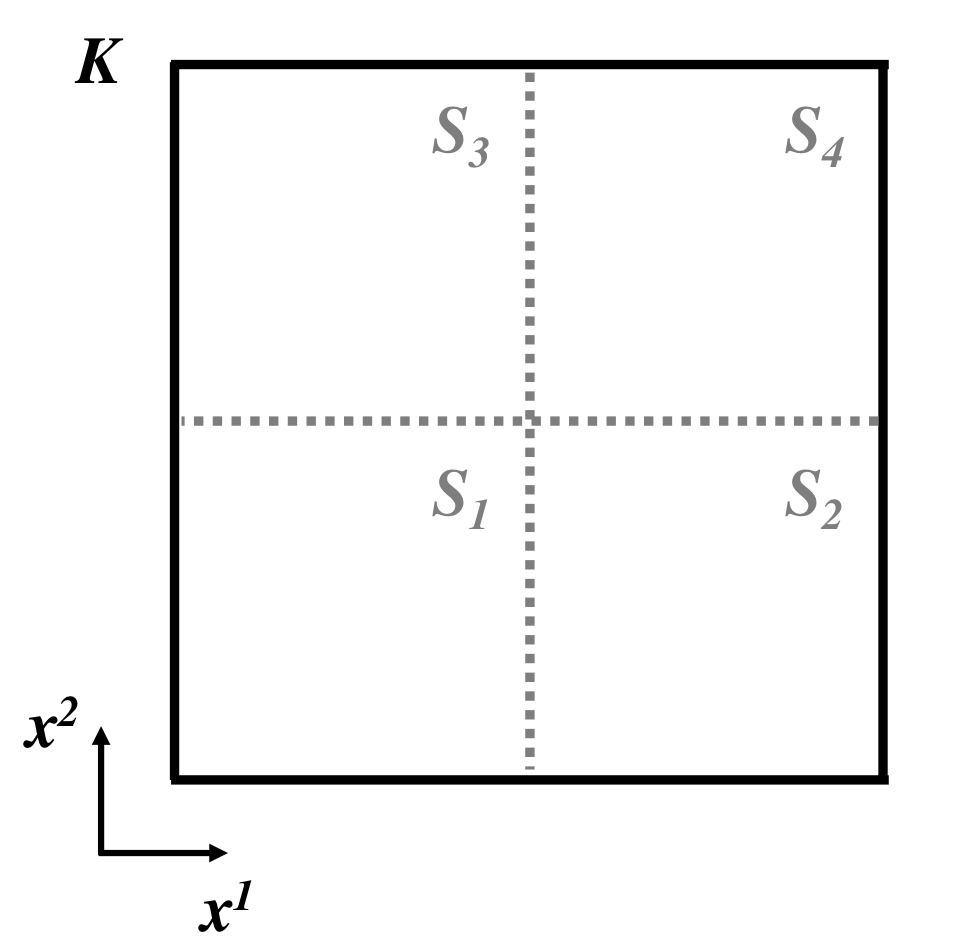
\includegraphics[width=0.75\textwidth]{./ElementSubgrid}
   \caption{Division of an element $\vect{K}$ into a subgrid of finite volume cells in two spatial dimensions ($d=2$) using DG polynomials of maximal degree $k=1$.}
  \label{fig:ElementSubgrid}
\end{figure}

\section{FV to DG Representation (Reconstruction)}

Knowing the cell averages $v_{j}$ (we suppress time dependence from here on), we reconstruct the DG representation $u_{h}$ by requiring that
\begin{equation}
  \f{1}{|S_{i}|}\int_{S_{i}}u_{h}(\vect{x})\,d\vect{x}
  =\f{1}{|S_{i}|}\int_{S_{i}}v_{h}(\vect{x})\,d\vect{x}=v_{i}, \forall~S_{i}\in S.
\end{equation}
With the definition in Eq.~\eqref{eq:dgRepresentation}, this gives
\begin{equation}
  R^{-1}\,\vect{u} = \vect{v},
\end{equation}
where $\vect{u}=(u_{1},\ldots,u_{(k+1)^{d}})^{T}$, $\vect{v}=(v_{1},\ldots,v_{(k+1)^{d}})^{T}$, and the components of the $(k+1)^{d}\times(k+1)^{d}$ inverse reconstruction matrix are
\begin{equation}
  R_{ij}^{-1}=\f{1}{|S_{i}|}\int_{S_{i}}\Phi_{j}(\vect{x})\,d\vect{x}.  
\end{equation}
The reconstruction step amounts inverting to find
\begin{equation}
  \vect{u} = R\,\vect{v}.
\end{equation}

\section{DG to FV Representation (Projection)}

Knowing the DG representation $u_{h}(\vect{x})$, we can easily compute the cell averages for the finite volume representation
\begin{equation}
  v_{i} = \f{1}{|S_{i}|}\int_{S_{i}}\,u_{h}(\vect{x})\,d\vect{x} = \f{1}{|S_{i}|}\sum_{j=1}^{(k+1)^{d}}\int_{S_{i}}\Phi_{j}(\vect{x})\,d\vect{x}\,u_{j},
\end{equation}
which can be written as
\begin{equation}
  \vect{v} = P\,\vect{u},
\end{equation}
where the components of the $(k+1)^{d}\times(k+1)^{d}$ projection matrix $P$ are
\begin{equation}
  P_{ij} = \f{1}{|S_{i}|}\int_{S_{i}}\Phi_{j}(\vect{x})\,d\vect{x}.  
\end{equation}
From the definitions above, it is obvious that $R\,P = I$; i.e., we do not lose any accuracy when switching between DG and FV representations.  
The reconstruction and projection matrices are plotted in Figure~\ref{fig:matrices} for $d=2$, $k=1$.  
\begin{figure}
  \centering
  \begin{tabular}{cc}
    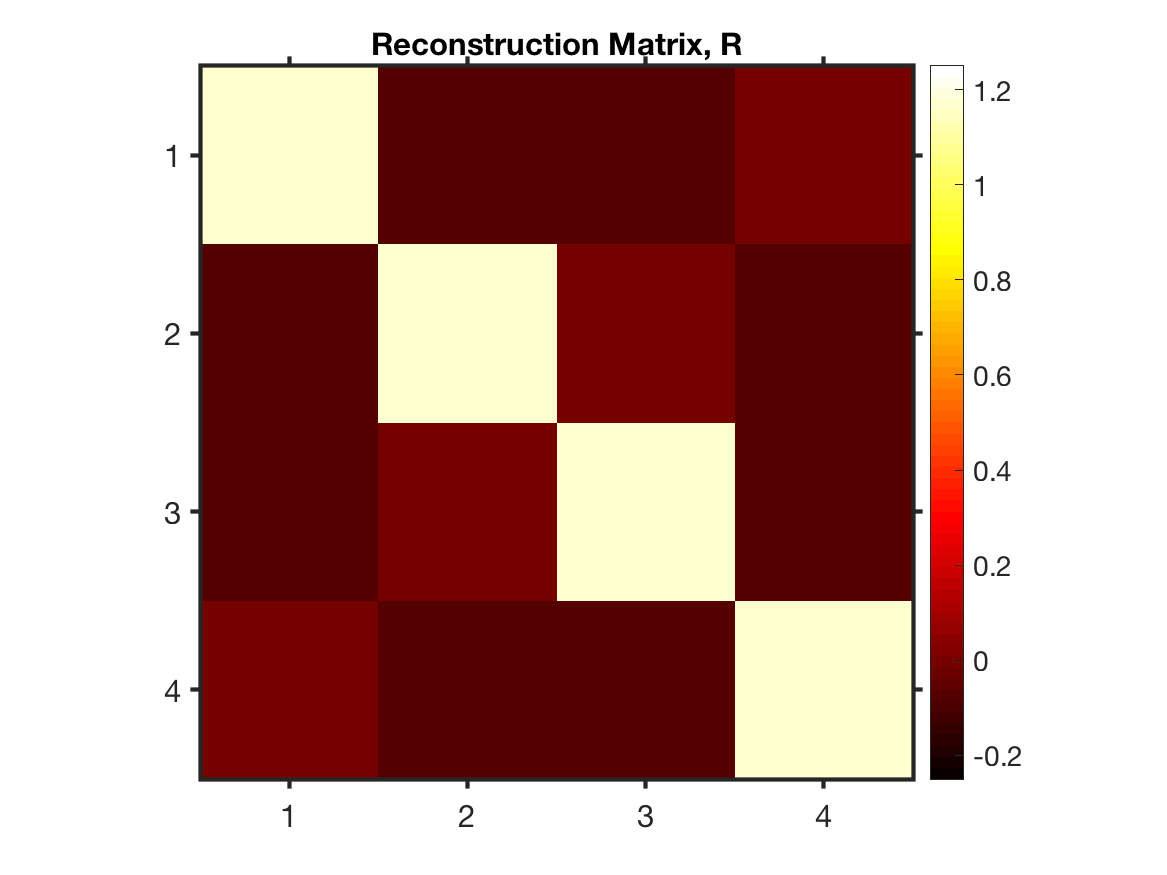
\includegraphics[width=0.5\textwidth]{./ReconstructionMatrix} &
    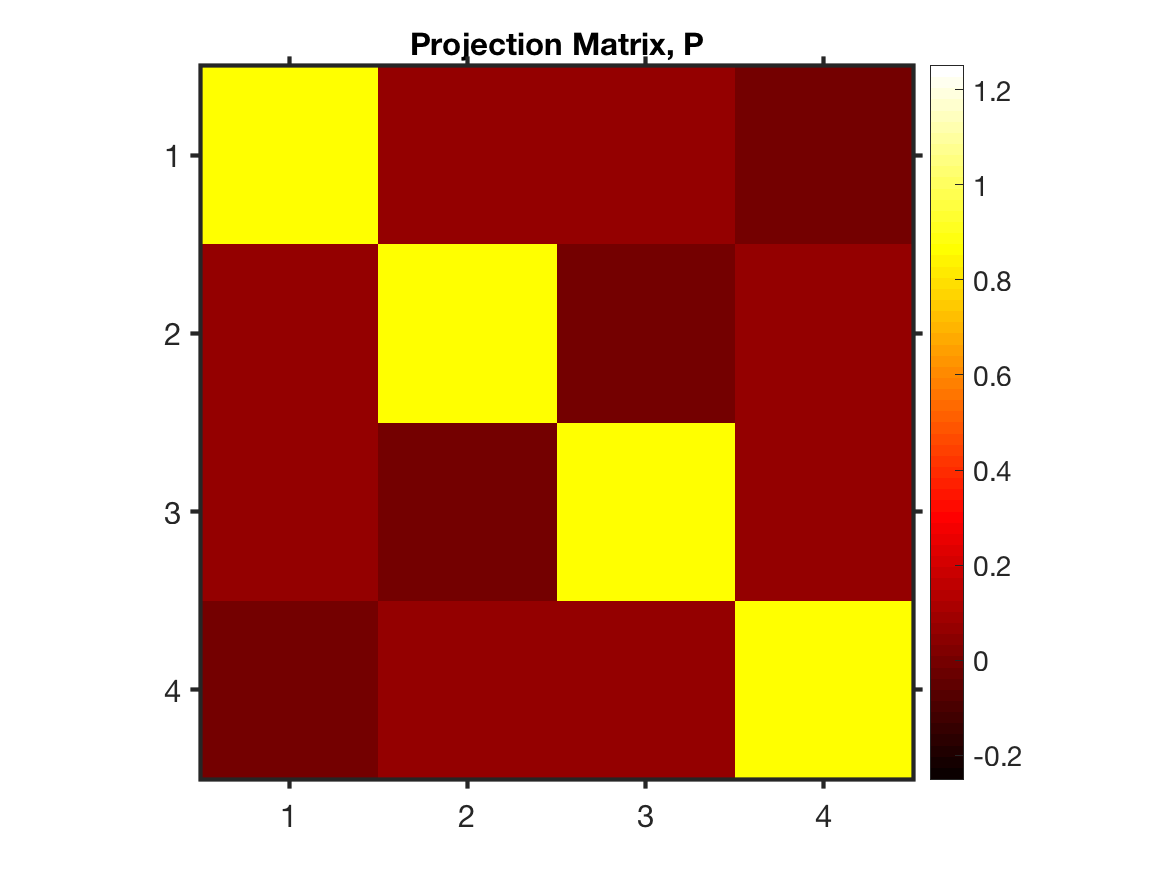
\includegraphics[width=0.5\textwidth]{./ProjectionMatrix}
  \end{tabular}
   \caption{Reconstruction matrix $R$ (left) and projection matrix $P$ for two spatial dimensions ($d=2$) using DG polynomials of maximal degree $k=1$.}
  \label{fig:matrices}
\end{figure}

\end{document}